\documentclass[a4paper,12pt]{report}
\usepackage[T1]{fontenc}
\usepackage[utf8]{inputenc}
\usepackage{lmodern}
\usepackage{amsmath}
\usepackage{amsfonts}
\usepackage{amssymb}
\usepackage{amsthm}
\usepackage{graphicx}
\usepackage{color}
\usepackage{xcolor}
\usepackage{url}
\usepackage{textcomp}
\usepackage{parskip}



\title{Implémentation d'une application de gestion de tache}
%\author{NKWE AHOUME BORIS}
\author{
  M. FOKOU KEMEGNE - Encadreur Académique\\
  %\texttt{first1.last1@xxxxx.com}
  \and
  M. HANNIEL TSASSE - Encadreur Professionel(FAROTY S.A.S)\\
  \and
  NKWE AHOUME BORIS - Etudiant en Genie Logiciel\\
  \texttt{nkabo074@gmail.com}
}


\date{\today}

\begin{document}

\vspace{0.06cm}

% Where the title will be.
\maketitle

% Where the table of contents will be.
\tableofcontents

% definie le titre du chapitre en FR
\def\chaptername{Chapitre} 

\renewcommand{\abstractname}{Dedicace}
\begin{abstract}
À mes parents, qui m'ont toujours soutenu et encouragé à poursuivre mes rêves. Merci de croire en moi.
\end{abstract}

\renewcommand{\abstractname}{Remerciment}
\begin{abstract}
Je souhaite exprimer ma profonde gratitude à toutes les personnes qui ont contribué à la réalisation de ce mémoire. Tout d'abord, je remercie Dieu Tout-Puissant pour m'avoir accordé la force, la sagesse et la persévérance nécessaires pour mener à bien ce projet.
Je tiens à remercier chaleureusement:

\begin{itemize}
  \item[•] le Directeur de l'Université pour le soutien institutionnel et les opportunités académiques offertes tout au long de mon parcours. Mes remerciements vont également au Responsable Académique, dont les conseils avisés et le dévouement ont été précieux.
  \item[•] mes parents, pour leur amour inconditionnel, leur soutien moral et financier, et leurs encouragements constants qui ont été une source inestimable de motivation.
  \item[•] mes frères et sœurs, je suis reconnaissant pour leur soutien affectueux et leur compréhension durant les moments difficiles.
  \item[•] mon Encadreur Professionnel M. HANNIEL TSASSE, dont l'expertise et les conseils pratiques m'ont guidé tout au long de cette recherche. 
  \item[•]Mon Encadreur Académique M. FOKOU KEMEGNE mérite aussi une reconnaissance particulière pour son accompagnement pédagogique, sa patience et ses précieux conseils.
\end{itemize}

Un grand merci à 
Je remercie également

\begin{itemize}
  \item[•] mes professeurs, qui ont partagé leur savoir et leur passion, contribuant ainsi de manière significative à ma formation.
  \item[•] merci sincère à mes camarades, pour leur soutien, leur camaraderie et les moments partagés qui ont rendu cette expérience mémorable et enrichissante.
\end{itemize}

À vous tous, merci infiniment.
\end{abstract}


\renewcommand{\abstractname}{Résumé}
\begin{abstract}
Le présent rapport détaille la conception et le développement d'une application de gestion de tâches, nommée GETDO pour le compte de la société FAROTY SAS. L'objectif principal de cette application est d'aider les utilisateurs à organiser efficacement leurs tâches quotidiennes, à suivre leur progression et à améliorer leur productivité.
L'application propose plusieurs fonctionnalités clés, notamment l'assignation de tâches avec des dates d'échéance, un tri en fonction des priorités, des rappels,un calendrier, un suivi de l'accomplissement des tâches, un tableau de vision pour visualiser les objectifs à long terme, ainsi qu'un tableau de bord offrant une vue d'ensemble de la progression des tâches à l'aide de graphiques.
Le développement de l'application s'est appuyé sur des technologies modernes telles que Vue JS pour le front-end et FireBase pour le back-end, offrant ainsi une expérience utilisateur fluide et intuitive. De plus,l'application fonctionnalités avancées telles que une optimisation de la planification et une analyse de productivité.
Ce rapport décrit en détail le processus de conception, de développement et de test de l'application, ainsi que les défis rencontrés et les solutions apportées. En outre, il met en évidence les perspectives d'amélioration et les pistes pour de futures recherches et développements dans le domaine de la gestion de tâches et des possibilité de l'intégration de l'Intelligence Artificielle.
En conclusion, l'application GETDO représente une contribution significative dans le domaine de la gestion de tâches, offrant aux utilisateurs une solution moderne et efficace pour gérer leur travail et améliorer leur productivité au quotidien.
\end{abstract}

% Introduction générale
\chapter*{Introduction Générale}
Dans un monde où le temps et les ressources sont des éléments précieux, la gestion efficace des tâches et des projets revêt une importance capitale pour les individus et les organisations. Dans ce contexte, les applications de gestion de tâches jouent un rôle essentiel en offrant des outils et des fonctionnalités permettant de planifier, suivre et organiser les activités quotidiennes et les projets à long terme de manière efficace et méthodique.
Le présent rapport détaille le processus de conception et de développement d'une application de gestion de tâches moderne, intitulée GETDO. Notre objectif principal est de fournir aux utilisateurs une solution robuste et intuitive pour gérer leurs tâches personnelles et professionnelles, en mettant l'accent sur l'optimisation de la productivité, la facilitation de la collaboration et l'amélioration de l'efficacité opérationnelle.
Ce rapport présentera en détail les différentes phases du projet, depuis la phase de conception initiale jusqu'au déploiement final de l'application. Nous aborderons les aspects techniques, fonctionnels et conceptuels du développement, en mettant en lumière les défis rencontrés, les solutions apportées et les choix technologiques effectués tout au long du processus.
De plus, nous explorerons les opportunités offertes par l'intégration de l'intelligence artificielle dans notre application, en examinant comment les fonctionnalités avancées telles que les recommandations intelligentes, l'analyse de données et l'automatisation peuvent contribuer à améliorer l'expérience utilisateur et à optimiser la gestion des tâches.
Enfin, nous discuterons des perspectives d'avenir pour notre application, en identifiant les pistes pour de futures améliorations, les évolutions technologiques envisagées et les possibilités d'extension et d'adaptation pour répondre aux besoins changeants des utilisateurs et du marché.
À travers ce rapport, nous espérons fournir un aperçu complet de notre travail et de notre vision pour l'application GETDO, ainsi que de son potentiel à contribuer à l'efficacité et à la réussite des individus et des organisations dans leur gestion quotidienne des tâches et des projets.

% presentation de l'entreprise
\chapter{Présentation de l'entreprise FAROTY SAS} 
FAROTY SAS est une société camerounaise innovante qui offre des solutions financières numériques à une clientèle grandissante. Localiser a près de l’hôtel Kremlin a Bonamousadi, FAROTY a pour mission de faciliter l'accès aux services financiers de base pour tous les Camerounais, en particulier ceux des zones rurales et non bancarisées.
FAROTY propose une suite complète de solutions financières numériques, notamment :
\begin{itemize}
\item[•] Paiements et transferts d'argent : Envoyez et recevez de l'argent facilement et en toute sécurité via des plateformes de paiement mobile et électronique (Orange Money, MTN Mobile Money, PayPal). 
\item[•] Gestion financière personnelle : Gérez vos finances personnelles en toute simplicité avec nos outils de budgétisation, de suivi des dépenses et d'épargne. 
\item[•] Collecte de fonds (Crowdfunding) : Levez des fonds pour vos projets et causes grâce à notre plateforme de crowdfunding sécurisée. 
\item[•] Tontines digitales : Participez à des tontines virtuelles et gérez vos cotisations en ligne. 
\item[•] Billetterie électronique : Achetez et vendez des billets d'événements en ligne avec notre service ePass. 
\item[•] Pages commerciales : Créez votre propre boutique en ligne et vendez vos produits et services facilement. 
Leurs technologie
\end{itemize} 
FAROTY a un impact positif sur les Camerounais en leur offrant un accès plus facile aux services financiers il est donc de notre devoir de facilité leurs travails via l'application présenter dans ce rapport

% Presentationde de l'equiment utiliser, et des methodes
\chapter{Méthode et equipements utilisé}
\section{équipement et logiciel utiliser}

Pour mener à bien ce projet, plusieurs outils technologiques ont été utilisés. Voici les principaux :
\begin{itemize}
\item IDE : Visual Studio Code a été l'éditeur de choix pour notre project.
\item Syteme de controle de version : Git.
\item Langages de Programmation : JavaScript pour front-end(Vue.JS) et FireBase en back-end
\end{itemize}

\section{Méthode utilisé}
Comme méthode utiliser, nous avont opter pour la méthode de dévélopement agile SCRUM et la modelisation UML. Chaque tâches sont séparé en sprint, et à la fin de chacun d'entre eux, un livrable est fournie. La liste des livrables et de l'application elle meme attendues pour ce project sont:
\begin{itemize}
  \item L'Application de gestion de tâche GETDO.
  \item Creation de tâche.
  \item Vision Board.
  \item Tableaux de bord et visualisations de données.
  \item Prise en charge d'un styles de gestion des tâches.
\end{itemize}

\subsection{Mise en place des outils de gestion de project}
Pour assuré la gestion bonne gestion du project, nous allons utiliser le logiciel de gestion JIRA

% Jira screenshot 
\begin{figure}[h!]
    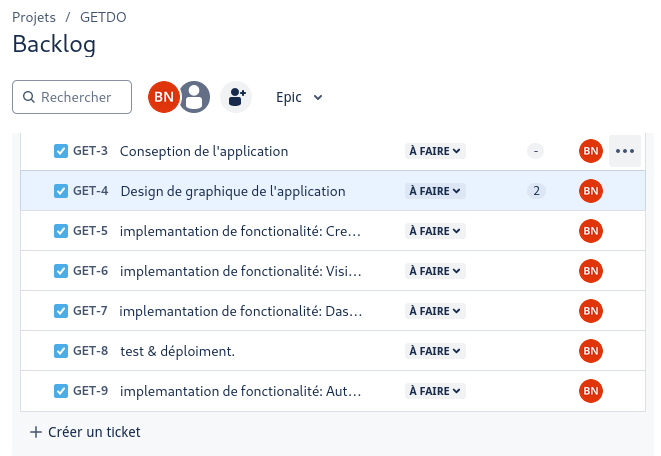
\includegraphics[width=1\textwidth]{./images/jira_project_task.png}
    \caption{Vue d'ensemble d'une tâche dans un projet Jira}
    \label{fig:jira_project_task}
\end{figure}
%---
\subsection{Conseption du project}
\subsubsection{Diagramme de cas d'utilisation et description textuelle}
Dans l'optique d'offire une experience utilisateur cohérante, nous nous devons de representer les diverses intéractions que l'utilisateur aura avec la plate forme. C'est pour cela que nous avons opter pour le diagramme de cas d'utilisation suivant: \\ \\ \\ \\ \\ \\ \\

% Use case diagramm screenshot
\begin{figure}[h!]
    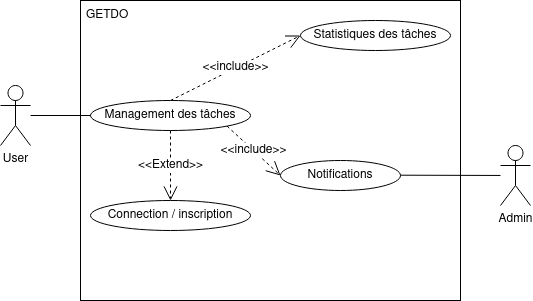
\includegraphics[width=1\textwidth]{./images/Diagramme_useCase.drawio.png}
    \caption{Diagramme de cas d'utilisation de GETDO}
    \label{fig:GETDO_UseCaseDiagramm}
\end{figure}
%---

% usecase diagramm description
\textbf{Système:} Système de gestion de tâches\\
\textbf{Acteurs:}
\begin{itemize}
    \item Utilisateur: Utilise le système pour créer, gérer et suivre ses tâches.
    \item Administrateur: Gère les utilisateurs, les paramètres du système et les rapports.
\end{itemize}
\textbf{Cas d'utilisation:}
\begin{itemize}
    \item Connexion/Inscription: L'utilisateur se connecte ou crée un compte.
    \item Gestion des tâches:
        L'utilisateur crée, modifie, supprime et organise ses tâches.
    \item Statistiques des tâches: L'utilisateur génère des rapports (tâches terminées, temps passé, tâches en retard).
    \item Notifications: L'utilisateur consulte les notifications envoyer par l'administrateur
\end{itemize}
\textbf{Relations:}
\begin{itemize}
    \item Utilisateur: Peut utiliser tous les cas d'utilisation.
    \item Administrateur: Peut envoyer des notifications a l'utilisateur.
    \item Gestion des tâches: Inclut les notifications.
    \item Statistiques des tâches: Étend la gestion des tâches.
\end{itemize}

\subsubsection{Senario de cas d'utilisation}

\textbf{Scénario utilisateur:} Création d'une tâche\\
\textbf{Acteur:} Utilisateur\\
\textbf{Cas d'utilisation:} Gestion des tâches\\
\textbf{Objectif:} Créer une nouvelle tâche dans le système.\\

\textbf{Étapes:}
\begin{itemize}
    \item L'utilisateur se connecte au système en utilisant son nom d'utilisateur et son mot de passe.
    \item L'utilisateur sélectionne l'option "Créer une tâche" dans le menu principal.
    \item L'utilisateur entre le titre de la tâche, une description détaillée, la date d'échéance et la priorité de la tâche.
    \item L'utilisateur clique sur le bouton "Enregistrer" pour créer la tâche.
    \item Le système enregistre la tâche et affiche un message de confirmation.
    \item L'utilisateur peut ensuite visualiser la tâche dans sa liste de tâches ou dans son calendrier.
\end{itemize}
\textbf{Variations:}
    L'utilisateur peut définir une date de rappel pour la tâche.
\textbf{Résultat:}
    Une nouvelle tâche est créée dans le système et est visible pour l'utilisateur qui l'a créée et pour les utilisatePlaurs auxquels elle a été attribuée.\\
%---

% Use case plot
\textbf{Scénario utilisateur:} Modification d'une tâche\\
\textbf{Acteur:} Utilisateur\\
\textbf{Cas d'utilisation:} Gestion des tâches\\
\textbf{Objectif:} Modifier une tâche existante dans le système.\\
\textbf{Étapes:}
\begin{itemize}
    \item L'utilisateur se connecte au système en utilisant son nom d'utilisateur et son mot de passe.
    \item L'utilisateur sélectionne la tâche qu'il souhaite modifier dans sa liste de tâches ou dans son calendrier.
    \item L'utilisateur modifie les informations de la tâche, telles que le titre, la description, la date d'échéance, la priorité, les étiquettes, les pièces jointes et les commentaires.
    \item L'utilisateur clique sur le bouton "Enregistrer" pour enregistrer les modifications.
    \item Le système enregistre les modifications et affiche un message de confirmation.
    \item Les modifications de la tâche sont reflétées dans la liste des tâches de l'utilisateur et dans le calendrier.
\end{itemize}
Variations:
\begin{itemize}
    \item L'utilisateur peut modifier l'état de la tâche, par exemple de "En cours" à "Terminée".
    \item L'utilisateur peut modifier la date de rappel de la tâche.
\end{itemize}
\textbf{Résultat:}
    La tâche est modifiée dans le système et les modifications sont reflétées pour tous les utilisateurs qui peuvent voir la tâche.\\

\textbf{Scénario utilisateur:} Suppression d'une tâche\\
\textbf{Acteur:} Utilisateur\\
\textbf{Cas d'utilisation:} Gestion des tâches\\
\textbf{Objectif:} Supprimer une tâche existante du système.\\
\textbf{Étapes:}
\begin{itemize}
    \item L'utilisateur se connecte au système en utilisant son nom d'utilisateur et son mot de passe.
    \item L'utilisateur sélectionne la tâche qu'il souhaite supprimer dans sa liste de tâches ou dans son calendrier.
    \item L'utilisateur clique sur le bouton "Supprimer" pour supprimer la tâche.
    \item Le système affiche une confirmation demandant à l'utilisateur de confirmer la suppression.
    \item L'utilisateur clique sur le bouton "Confirmer" pour supprimer définitivement la tâche.
    \item Le système supprime la tâche et affiche un message de confirmation.
\end{itemize}
Résultat:
    La tâche est supprimée du système et n'est plus visible pour les utilisateurs.
%---

\subsection{Identité visuelle du project}
L'identité visuelle est l'élément crucial qui donne vie à la personnalité et aux valeurs d'un projet. Elle constitue la première impression que les utilisateurs auront de votre application et joue un rôle essentiel dans la création d'une expérience utilisateur cohérente et engageante.

Cette section du plan de projet s'attache à définir les principes fondamentaux qui guideront la création de l'identité visuelle de l'application. Elle couvrira les aspects suivants :

\begin{itemize}
  \item \textbf{Logo et charte graphique:} Définir les éléments visuels clés qui représentent l'identité de l'application, tels que le logo, la palette de couleurs, la typographie et les images.
  
  \item \textbf {Directives de style:} Établir des règles claires et cohérentes pour l'utilisation de l'identité visuelle dans tous les supports de communication, y compris l'interface utilisateur, les documents marketing et les supports promotionnels.
\end{itemize}
\subsubsection{Logo et charte graphique}
Le logo et la charte graphique sont les piliers fondamentaux de l'identité visuelle d'un projet. Ils constituent la représentation visuelle de la marque et jouent un rôle crucial dans la communication des valeurs, de la mission et de la personnalité du projet auprès du public cible.

\begin{figure}[h!]
    
\includegraphics[width=1\textwidth]{./images/GETDO_logo.png}
    \caption{Logo de GETDO......}
    \label{fig:jira_project_task}
\end{figure}

\end{document}